Haizea is an open-source VM-based lease management architecture. Let's break that down, shall we?

\begin{description}
\item[Haizea is a resource manager] (or, depending on who you ask, a "resource scheduler"): Haizea is a software component that can manage a set of computers (typically a cluster), allowing users to request exclusive use of those resources described in a variety of terms, such as "I need 10 nodes, each with 1 GB of memory, right now" or "I need 4 nodes, each with 2 CPUs and 2GB of memory, from 2pm to 4pm tomorrow".
\item[Haizea uses leases] The fundamental resource provisioning abstraction in Haizea is the lease. Intuitively, a lease is some form of contract where one party agrees to provide a set of resources (an apartment, a car, etc.) to another party. When a user wants to request computational resources from Haizea, it does so in the form of a lease. When applied to computational resources, the lease abstraction is a powerful and general construct with a lot of nuances. See below for a more detailed definition of leases or read about the types of leases supported by Haizea.
\item[Haizea is VM-based] We hold that the best way of implementing resource leases is using virtual machines (VMs). Therefore, Haizea's scheduling algorithms are geared towards managing virtual machines, factoring in all the extra operations (and overhead) involved in managing VMs. The Globus Virtual Workspaces group, where Haizea was originally developed, has an extensive list of publications that argue how using virtual machines for resource leasing is A Good Thing (and also Not A Trivial Thing).
\item[Haizea is open source] Haizea is published under the Apache License 2.0, a BSD-like OSI-compatible license.
\end{description}

\section{What can you do with Haizea?}

\begin{center}
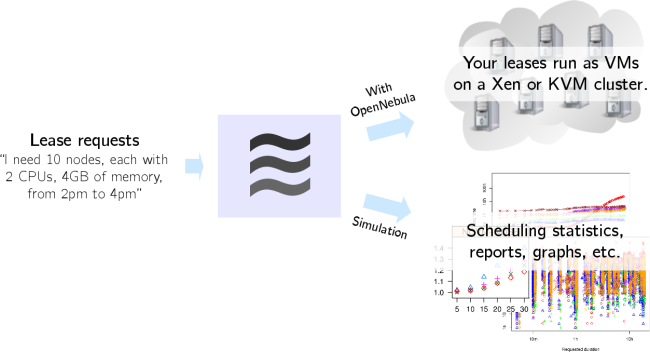
\includegraphics{images/what_haizea_does.png}
\end{center}


You can use Haizea one of two ways. Haizea can be used as a standalone component or as a scheduling backend for a virtual infrastructure manager, such as OpenNebula. So, if you're...

\begin{description}
\item[Using Haizea with OpenNebula] Haizea can be used as a drop-in replacement for OpenNebula's scheduling daemon. OpenNebula is a virtual infrastructure manager that enables the dynamic deployment and re-allocation of virtual machines on a pool of physical resources. OpenNebula and Haizea complement each other, since OpenNebula provides all the enactment muscle (OpenNebula can manage Xen and KVM virtual machines on a cluster, with VMWare support to follow shortly) while Haizea provides all the scheduling brains. The document "Using OpenNebula and Haizea to manage VMs on a cluster" provides more details on how to use OpenNebula 1.0 and Haizea together.
\item[Using Haizea on its own] In this case, you actually can't do all that much :-) Haizea is, primarily, a VM resource management component that can take lease requests and make scheduling decisions, but doesn't actually know anything about how to enact those decisions. For example, Haizea may determine at what times a set of VMs representing a lease must start and stop, but it doesn't actually know how to instruct a virtual machine manager to do these actions. Haizea can, however, simulate those enactment actions so, on its own, Haizea might be useful if you're doing scheduling research involving leases or VMs (in fact, the Haizea simulator has been used in a couple of papers).
\end{description}

You can find a couple (more specific) details about what you can do with Haizea in our list of features.

\section{Leasing as a fundamental abstraction}

Let's say you need computational resources...

Maybe you're a scientist who needs to run some simulations. You have specific hardware requirements, but you're not particularly picky about when the simulations run, and probably won't even notice if they are interrupted at some point, as long as they finish running (correctly) at some point, maybe before a given deadline. A job scheduler, and a compute cluster, would probably be a good fit for you.

You could also be a software developer who wants to test his or her code on a pristine machine, which you would only need for a relatively short period of time. Plus, every time you use this machine, you'd like it to start up with the exact same pristine software environment. Oh, and you want your machine now. As in right now. One option could be to install a virtual machine (VM) manager (such as Xen, VMWare, etc.) to start up these pristine machines as VMs on your own machine. Even better, you could go to a cloud (like Amazon EC2 or the Science Clouds) and have those VMs appear automagically somewhere else, so you don't have to worry about setting up the VM manager or having a machine powerful enough to run those VMs.

Or perhaps you're a run-of-the-mill geek who wants his or her own web/mail/DNS/etc server. This server will presumably be running for months or even years with high availability: your server has to be running all the time, with no interruptions. There's a whole slew of hosting providers who can give you a dedicated server or a virtual private server. The latter are typically managed with VM-based datacenter managers.

As you can see, there are a lot of resource provisioning scenarios in nature. However, the solutions that have emerged tend to be specific to a particular scenario, to the exclusion of other ones. For example, while job-based systems are exceptionally good at managing complex batch workloads, they're not too good at provisioning resources at specific times (some job-based systems do offer advance reservations, but they have well-known utilization problems) or at giving users unfettered access to provisioned resources (forcing them, instead, to interact with the resources through the job abstraction).

A lease is a general resource provisioning abstraction that could be used to satisfy a variety of use cases, such as the ones described above. In our work, we've defined a lease as "a negotiated and renegotiable agreement between a resource provider and a resource consumer, where the former agrees to make a set of resource available to the latter, based on a set of lease terms presented by the resource consumer". In our view, the lease terms must include the following dimensions:

\begin{description}
 \item[Hardware] The hardware resources (CPU, memory, etc.) required by the resource consumer.
 \item[Software] The software environment that must be installed in those resources.
 \item[Availability] The period during which the hardware and software resources must be available. It is important to note that the availability period can be specified in a variety of ways, like "just get this to me as soon as you can", "I need this from 2pm to 4pm on Mondays, Wednesdays, and Fridays (and, if I don't get exactly this, I will be a very unhappy resource consumer)", or even "I need four hours sometime before 5pm tomorrow, although if you get the resources to me right now I'll settle for just two hours". A lease-based system must be able to efficiently combine all these different types of availability.
\end{description}

Furthermore, if you don't get any of these dimensions, then you're being shortchanged by your resource lessor. For example, Amazon EC2 is very good at providing exactly the software environment you want, and reasonably good at providing the hardware you want (although you're limited to a few hardware configurations), but not so good at supporting a variety of availability periods.

So, Haizea aims to support resource leasing along these three dimension. For now, Haizea supports three types of availability:

\begin{description}
\item[Best-effort lease] Resources are provisioned as soon as they are available.
\item[Advance reservation-style leases (or "AR leases")] Resources are provisioned during a strictly defined time period (e.g., from 2pm to 4pm).
\item[Immediate leases] Resources must be provisioned right now, or not at all.
\end{description}

Although there are many systems (particularly job-based systems) that support these two types availability, Haizea differs in that it efficiently schedules heterogeneous workloads (combining best-effort and AR leases), overcoming the utilization problems typically resulting from using ARs. Haizea does this by using virtual machines to implement leases. Virtual machines also enable Haizea to provide exactly the hardware and software requested by the user. Additionally, Haizea also manages the overhead of preparing a lease, to make sure that any deployment operations (such as transferring a VM disk image) are taken care of before the start of a lease, instead of being deducted from the lessee's allocation.

In the future, Haizea will support additional lease types, such as urgent leases, periodic leases, deadline-driven leases, etc.

\section{Features}

Foobar

\section{Haizea is extensible}

The Haizea architecture has been designed so it can be used as a scheduling component that can be plugged into other systems by implementing a set of extra modules in Haizea using a well-defined API (i.e., without having to modify the core of Haizea). Right now, Haizea depends on OpenNebula to perform enactment actions on real systems (and, in turn, OpenNebula can use Haizea as its scheduling backend), but Haizea could be made to work with other systems with relative ease. See the Haizea architecture page for more details.

\section{Haizea is still a technology preview}

Haizea started out as research software (and it is still largely meant for research purposes). Although Haizea works and we're getting to the point where it can be used in production systems, it is still a technology preview, so please use it with caution. In particular, although we've produced some documentation and polished up the code, there is still a fair amount of documentation that has to be produced. If you have any trouble using Haizea, or understanding any part of the source code, please don't hesitate to ask for help.